\documentclass{standalone}
\usepackage{tikz}
\usetikzlibrary{patterns, positioning}


\begin{document}
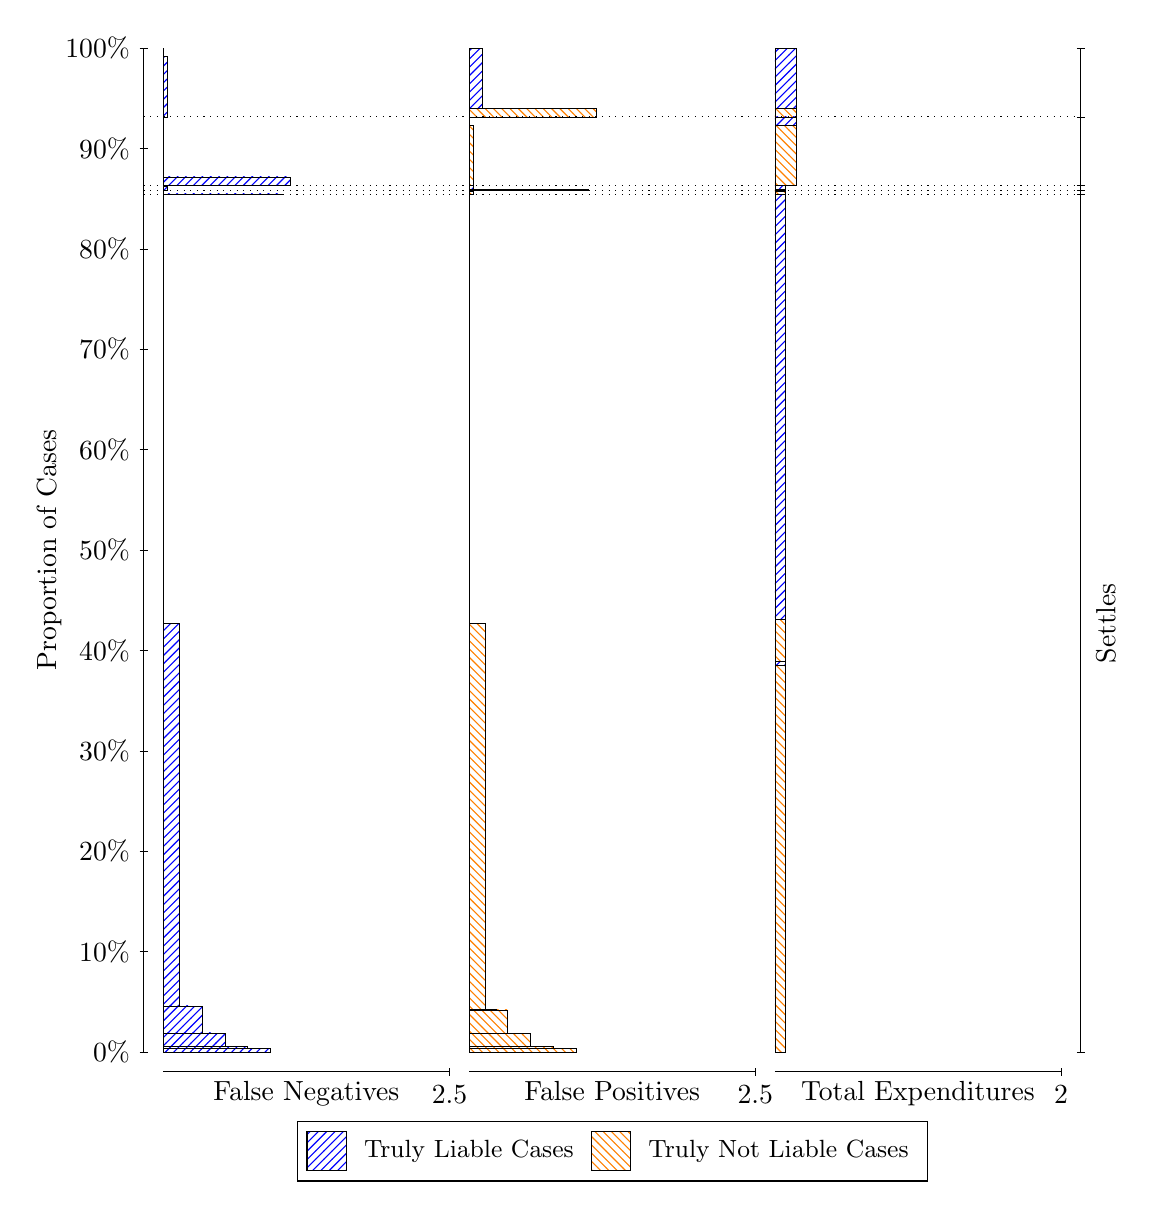
\begin{tikzpicture}
\draw[black, very thin] (1.5,1.75) -- (1.5,14.5);
\node[rotate=90, text=black, anchor=center] at (0.3, 8.125) {Proportion of Cases};
\draw[black, very thin] (1.45,1.75) -- (1.55,1.75);
\node[text=black, anchor=east] at (1.45, 1.75) {0\%};
\draw[black, very thin] (1.45,3.025) -- (1.55,3.025);
\node[text=black, anchor=east] at (1.45, 3.025) {10\%};
\draw[black, very thin] (1.45,4.3) -- (1.55,4.3);
\node[text=black, anchor=east] at (1.45, 4.3) {20\%};
\draw[black, very thin] (1.45,5.575) -- (1.55,5.575);
\node[text=black, anchor=east] at (1.45, 5.575) {30\%};
\draw[black, very thin] (1.45,6.85) -- (1.55,6.85);
\node[text=black, anchor=east] at (1.45, 6.85) {40\%};
\draw[black, very thin] (1.45,8.125) -- (1.55,8.125);
\node[text=black, anchor=east] at (1.45, 8.125) {50\%};
\draw[black, very thin] (1.45,9.4) -- (1.55,9.4);
\node[text=black, anchor=east] at (1.45, 9.4) {60\%};
\draw[black, very thin] (1.45,10.675) -- (1.55,10.675);
\node[text=black, anchor=east] at (1.45, 10.675) {70\%};
\draw[black, very thin] (1.45,11.95) -- (1.55,11.95);
\node[text=black, anchor=east] at (1.45, 11.95) {80\%};
\draw[black, very thin] (1.45,13.225) -- (1.55,13.225);
\node[text=black, anchor=east] at (1.45, 13.225) {90\%};
\draw[black, very thin] (1.45,14.5) -- (1.55,14.5);
\node[text=black, anchor=east] at (1.45, 14.5) {100\%};

\draw[black, very thin] (13.4,1.75) -- (13.4,14.5);
\draw[black, very thin] (13.35,1.75) -- (13.45,1.75);
\node[anchor=west] at (13.35, 1.75) {};
\draw[black, very thin] (13.35,12.639) -- (13.45,12.639);
\node[anchor=west] at (13.35, 12.639) {};
\draw[black, very thin] (13.35,12.696) -- (13.45,12.696);
\node[anchor=west] at (13.35, 12.696) {};
\draw[black, very thin] (13.35,12.752) -- (13.45,12.752);
\node[anchor=west] at (13.35, 12.752) {};
\draw[black, very thin] (13.35,13.626) -- (13.45,13.626);
\node[anchor=west] at (13.35, 13.626) {};
\draw[black, very thin] (13.35,14.5) -- (13.45,14.5);
\node[anchor=west] at (13.35, 14.5) {};

\draw[black, very thin, pattern color=blue, pattern=north east lines] (1.75,1.75) rectangle (3.1125,1.7989);
\draw[black, very thin, pattern color=blue, pattern=north east lines] (1.75,1.7989) rectangle (2.9672,1.7992);
\draw[black, very thin, pattern color=blue, pattern=north east lines] (1.75,1.7992) rectangle (2.8218,1.8214);
\draw[black, very thin, pattern color=blue, pattern=north east lines] (1.75,1.8214) rectangle (2.6765,1.8223);
\draw[black, very thin, pattern color=blue, pattern=north east lines] (1.75,1.8223) rectangle (2.5312,1.9862);
\draw[black, very thin, pattern color=blue, pattern=north east lines] (1.75,1.9862) rectangle (2.3858,1.9917);
\draw[black, very thin, pattern color=blue, pattern=north east lines] (1.75,1.9917) rectangle (2.2405,2.3328);
\draw[black, very thin, pattern color=blue, pattern=north east lines] (1.75,2.3328) rectangle (2.0952,2.3365);
\draw[black, very thin, pattern color=blue, pattern=north east lines] (1.75,2.3365) rectangle (1.9498,7.1944);
\draw[black, very thin, pattern color=orange, pattern=north west lines] (1.75,7.1944) rectangle (1.75,12.639);
\draw[black, very thin, pattern color=blue, pattern=north east lines] (1.75,12.639) rectangle (3.2578,12.648);
\draw[black, very thin, pattern color=orange, pattern=north west lines] (1.75,12.648) rectangle (1.75,12.696);
\draw[black, very thin, pattern color=blue, pattern=north east lines] (1.75,12.696) rectangle (1.8045,12.743);
\draw[black, very thin, pattern color=orange, pattern=north west lines] (1.75,12.743) rectangle (1.75,12.752);
\draw[black, very thin, pattern color=blue, pattern=north east lines] (1.75,12.752) rectangle (3.3668,12.863);
\draw[black, very thin, pattern color=orange, pattern=north west lines] (1.75,12.863) rectangle (1.75,13.626);
\draw[black, very thin, pattern color=blue, pattern=north east lines] (1.75,13.626) rectangle (1.8045,14.389);
\draw[black, very thin, pattern color=orange, pattern=north west lines] (1.75,14.389) rectangle (1.75,14.5);
\draw[black, very thin, pattern color=orange, pattern=north west lines] (5.6333,1.75) rectangle (6.9958,1.7951);
\draw[black, very thin, pattern color=orange, pattern=north west lines] (5.6333,1.7951) rectangle (6.8505,1.7954);
\draw[black, very thin, pattern color=orange, pattern=north west lines] (5.6333,1.7954) rectangle (6.7052,1.8211);
\draw[black, very thin, pattern color=orange, pattern=north west lines] (5.6333,1.8211) rectangle (6.5598,1.822);
\draw[black, very thin, pattern color=orange, pattern=north west lines] (5.6333,1.822) rectangle (6.4145,1.9855);
\draw[black, very thin, pattern color=orange, pattern=north west lines] (5.6333,1.9855) rectangle (6.2692,1.9861);
\draw[black, very thin, pattern color=orange, pattern=north west lines] (5.6333,1.9861) rectangle (6.2692,1.9897);
\draw[black, very thin, pattern color=orange, pattern=north west lines] (5.6333,1.9897) rectangle (6.1238,2.2832);
\draw[black, very thin, pattern color=orange, pattern=north west lines] (5.6333,2.2832) rectangle (5.9785,2.2882);
\draw[black, very thin, pattern color=orange, pattern=north west lines] (5.6333,2.2882) rectangle (5.8332,7.1949);
\draw[black, very thin, pattern color=blue, pattern=north east lines] (5.6333,7.1949) rectangle (5.6333,12.639);
\draw[black, very thin, pattern color=orange, pattern=north west lines] (5.6333,12.639) rectangle (5.6878,12.686);
\draw[black, very thin, pattern color=blue, pattern=north east lines] (5.6333,12.686) rectangle (5.6333,12.696);
\draw[black, very thin, pattern color=orange, pattern=north west lines] (5.6333,12.696) rectangle (7.1412,12.704);
\draw[black, very thin, pattern color=blue, pattern=north east lines] (5.6333,12.704) rectangle (5.6878,12.752);
\draw[black, very thin, pattern color=orange, pattern=north west lines] (5.6333,12.752) rectangle (5.6878,13.515);
\draw[black, very thin, pattern color=blue, pattern=north east lines] (5.6333,13.515) rectangle (5.6333,13.626);
\draw[black, very thin, pattern color=orange, pattern=north west lines] (5.6333,13.626) rectangle (7.2502,13.737);
\draw[black, very thin, pattern color=blue, pattern=north east lines] (5.6333,13.737) rectangle (5.7968,14.5);
\draw[black, very thin, pattern color=orange, pattern=north west lines] (9.5167,1.75) rectangle (9.6529,6.6617);
\draw[black, very thin, pattern color=blue, pattern=north east lines] (9.5167,6.6617) rectangle (9.6529,6.7109);
\draw[black, very thin, pattern color=orange, pattern=north west lines] (9.5167,6.7109) rectangle (9.6529,7.2441);
\draw[black, very thin, pattern color=blue, pattern=north east lines] (9.5167,7.2441) rectangle (9.6529,12.639);
\draw[black, very thin, pattern color=orange, pattern=north west lines] (9.5167,12.639) rectangle (9.6529,12.686);
\draw[black, very thin, pattern color=blue, pattern=north east lines] (9.5167,12.686) rectangle (9.6529,12.696);
\draw[black, very thin, pattern color=orange, pattern=north west lines] (9.5167,12.696) rectangle (9.6529,12.704);
\draw[black, very thin, pattern color=blue, pattern=north east lines] (9.5167,12.704) rectangle (9.6529,12.752);
\draw[black, very thin, pattern color=orange, pattern=north west lines] (9.5167,12.752) rectangle (9.7892,13.515);
\draw[black, very thin, pattern color=blue, pattern=north east lines] (9.5167,13.515) rectangle (9.7892,13.626);
\draw[black, very thin, pattern color=orange, pattern=north west lines] (9.5167,13.626) rectangle (9.7892,13.737);
\draw[black, very thin, pattern color=blue, pattern=north east lines] (9.5167,13.737) rectangle (9.7892,14.5);
\draw[black, dotted] (1.5,12.639) -- (13.4,12.639);
\draw[black, dotted] (1.5,12.696) -- (13.4,12.696);
\draw[black, dotted] (1.5,12.752) -- (13.4,12.752);
\draw[black, dotted] (1.5,13.626) -- (13.4,13.626);
\draw[black, very thin] (1.75,1.5) -- (5.3833,1.5);
\node[text=black, anchor=north] at (3.5667, 1.5) {False Negatives};
\draw[black, very thin] (5.3833,1.45) -- (5.3833,1.55);
\node[text=black, anchor=north] at (5.3833, 1.45) {2.5};

\draw[black, very thin] (5.6333,1.5) -- (9.2667,1.5);
\node[text=black, anchor=north] at (7.45, 1.5) {False Positives};
\draw[black, very thin] (9.2667,1.45) -- (9.2667,1.55);
\node[text=black, anchor=north] at (9.2667, 1.45) {2.5};

\draw[black, very thin] (9.5167,1.5) -- (13.15,1.5);
\node[text=black, anchor=north] at (11.333, 1.5) {Total Expenditures};
\draw[black, very thin] (13.15,1.45) -- (13.15,1.55);
\node[text=black, anchor=north] at (13.15, 1.45) {2};

\node[text=black, centered, rotate=90] at (13.72, 7.1947) {Settles};





\draw (7.449999999999999,1.5) node[draw=none] (baseCoordinate) {};
\begin{scope}[align=center]
        \matrix[scale=0.5, draw=black, below=0.5cm of baseCoordinate, nodes={draw}, column sep=0.1cm]{
            \node[rectangle, draw, minimum width=0.5cm, minimum height=0.5cm, pattern color=blue, pattern=north east lines] {}; &
            \node[draw=none, font=\small, text=black] (B) {Truly Liable Cases}; &
            \node[rectangle, draw, minimum width=0.5cm, minimum height=0.5cm, pattern color=orange, pattern=north west lines] {}; &
            \node[draw=none, font=\small, text=black] (B) {Truly Not Liable Cases}; \\
            };
\end{scope}

\end{tikzpicture}
\end{document}